%----------------------------------------------------------------------------
\appendix
%----------------------------------------------------------------------------
\chapter*{\fuggelek}\addcontentsline{toc}{chapter}{\fuggelek}
\setcounter{chapter}{\appendixnumber}
%\setcounter{equation}{0} % a fofejezet-szamlalo az angol ABC 6. betuje (F) lesz
\numberwithin{equation}{section}
\numberwithin{figure}{section}
\numberwithin{lstlisting}{section}
%\numberwithin{tabular}{section}

\begin{figure}[h]
    \centering
    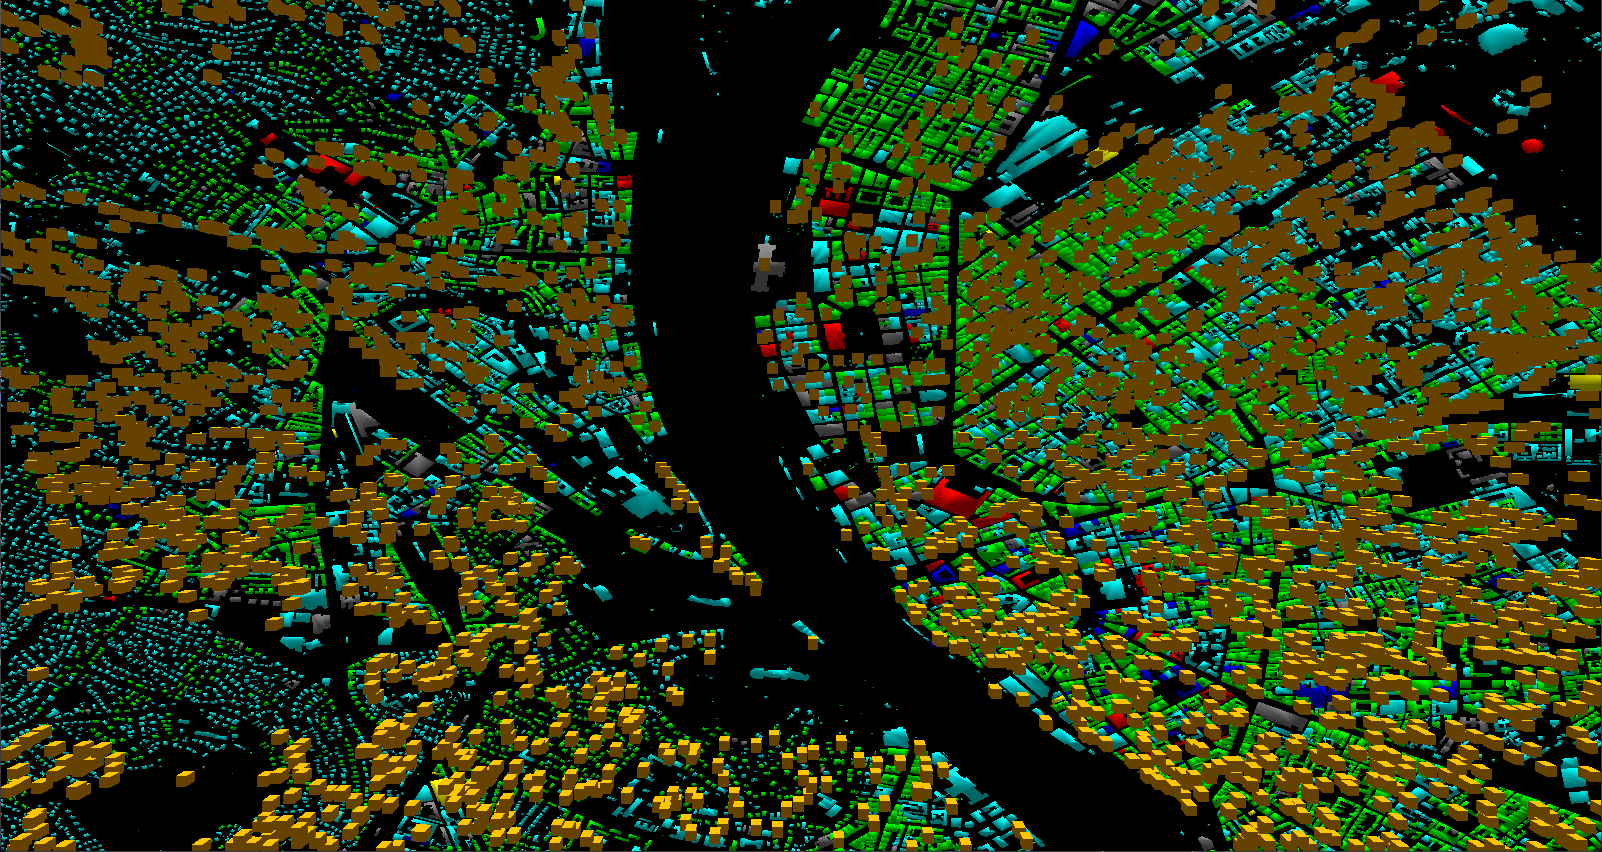
\includegraphics[width=140mm, keepaspectratio]{images/overlay_v1.png}
    \caption{An array of cubes displayed over the city of Budapest, each representing an agent; this was the first overlay version\ \label{overlay_v1}}
\end{figure}
\begin{figure}[h]
    \centering
    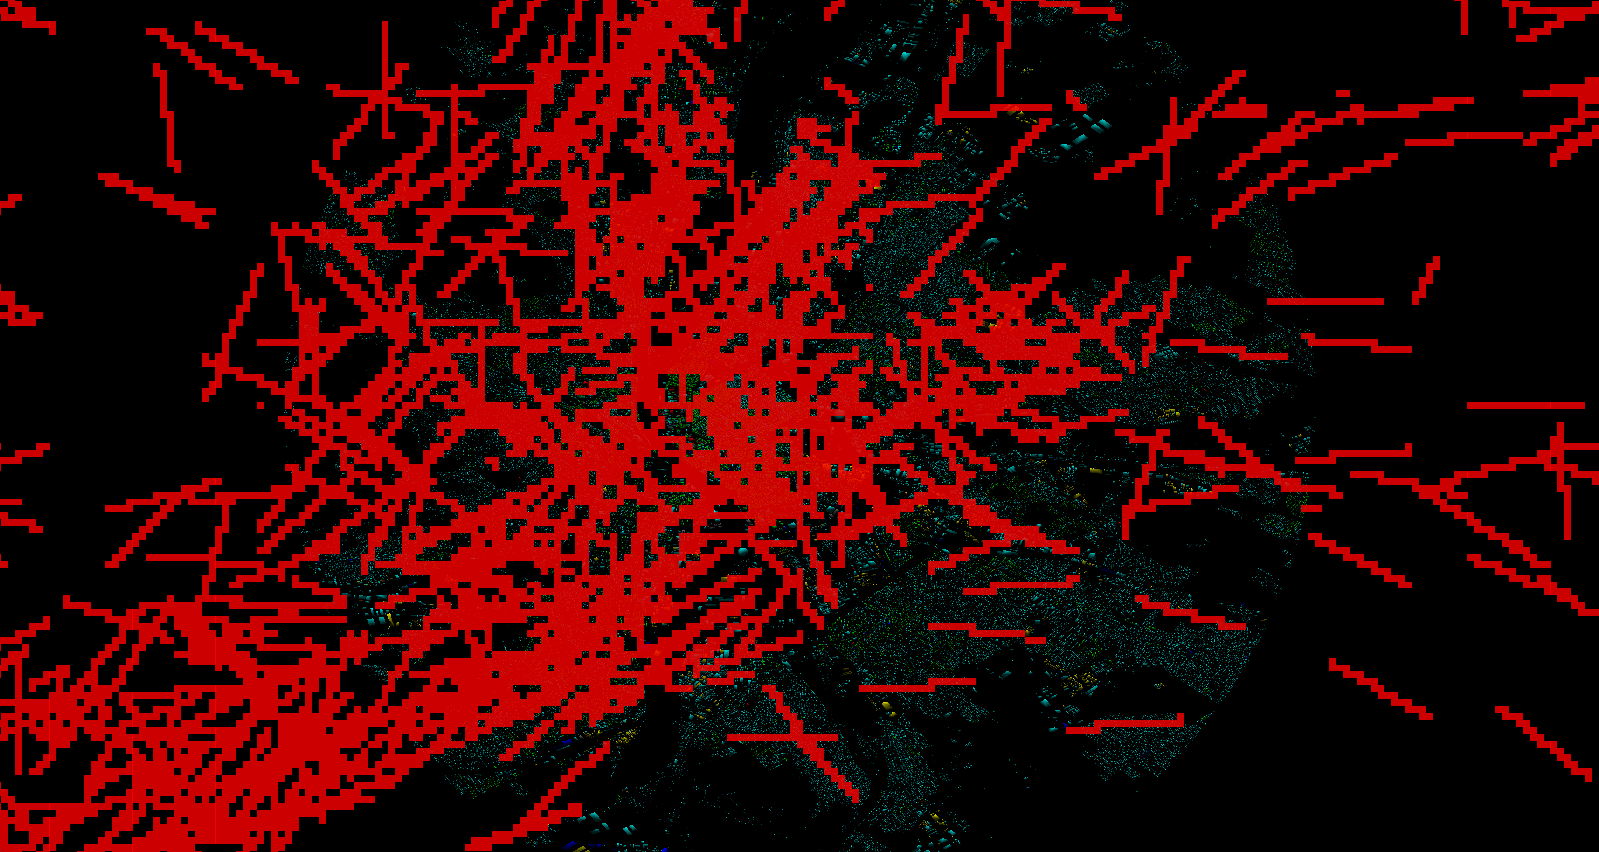
\includegraphics[width=140mm, keepaspectratio]{images/overlay_v2.png}
    \caption{An overlay with flattened opacity, displayed over the city of Budapest. Agent paths are randomised and are traversed in a straight line; this was the second overlay version\ \label{overlay_v2}}
\end{figure}

\label{comparison_heatmap}
\begin{figure}[h]
    \centering
    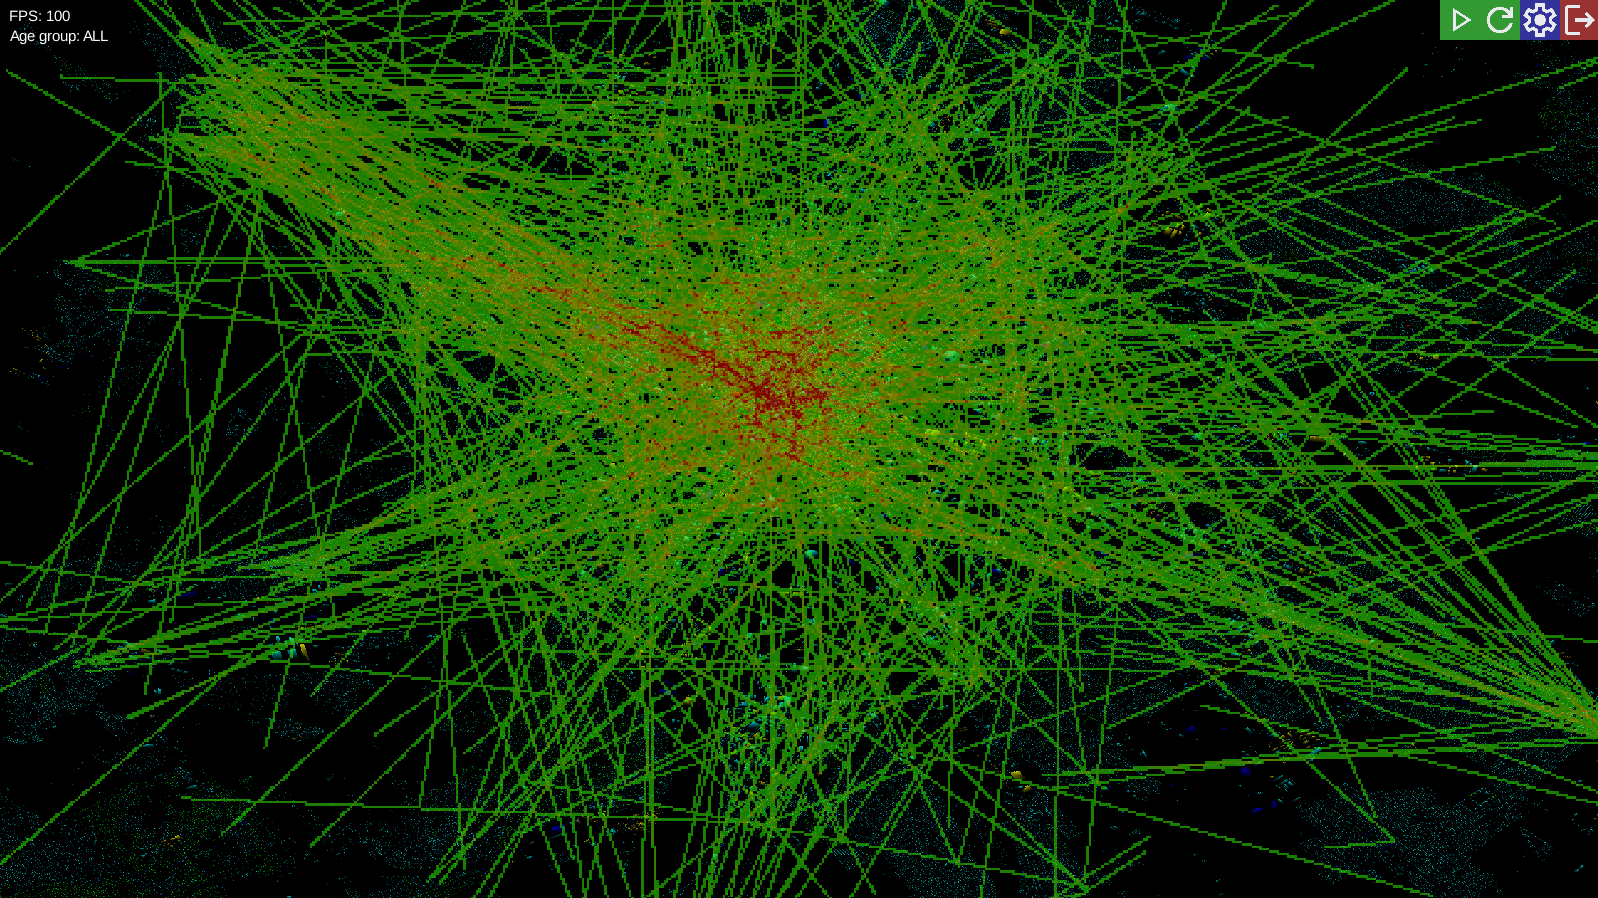
\includegraphics[width=140mm, keepaspectratio]{images/heatmap_1000.png}
    \caption{Heatmap using 1000 agents, see \ref{perftesting-heatmap}}
\end{figure}
\begin{figure}[h]
    \centering
    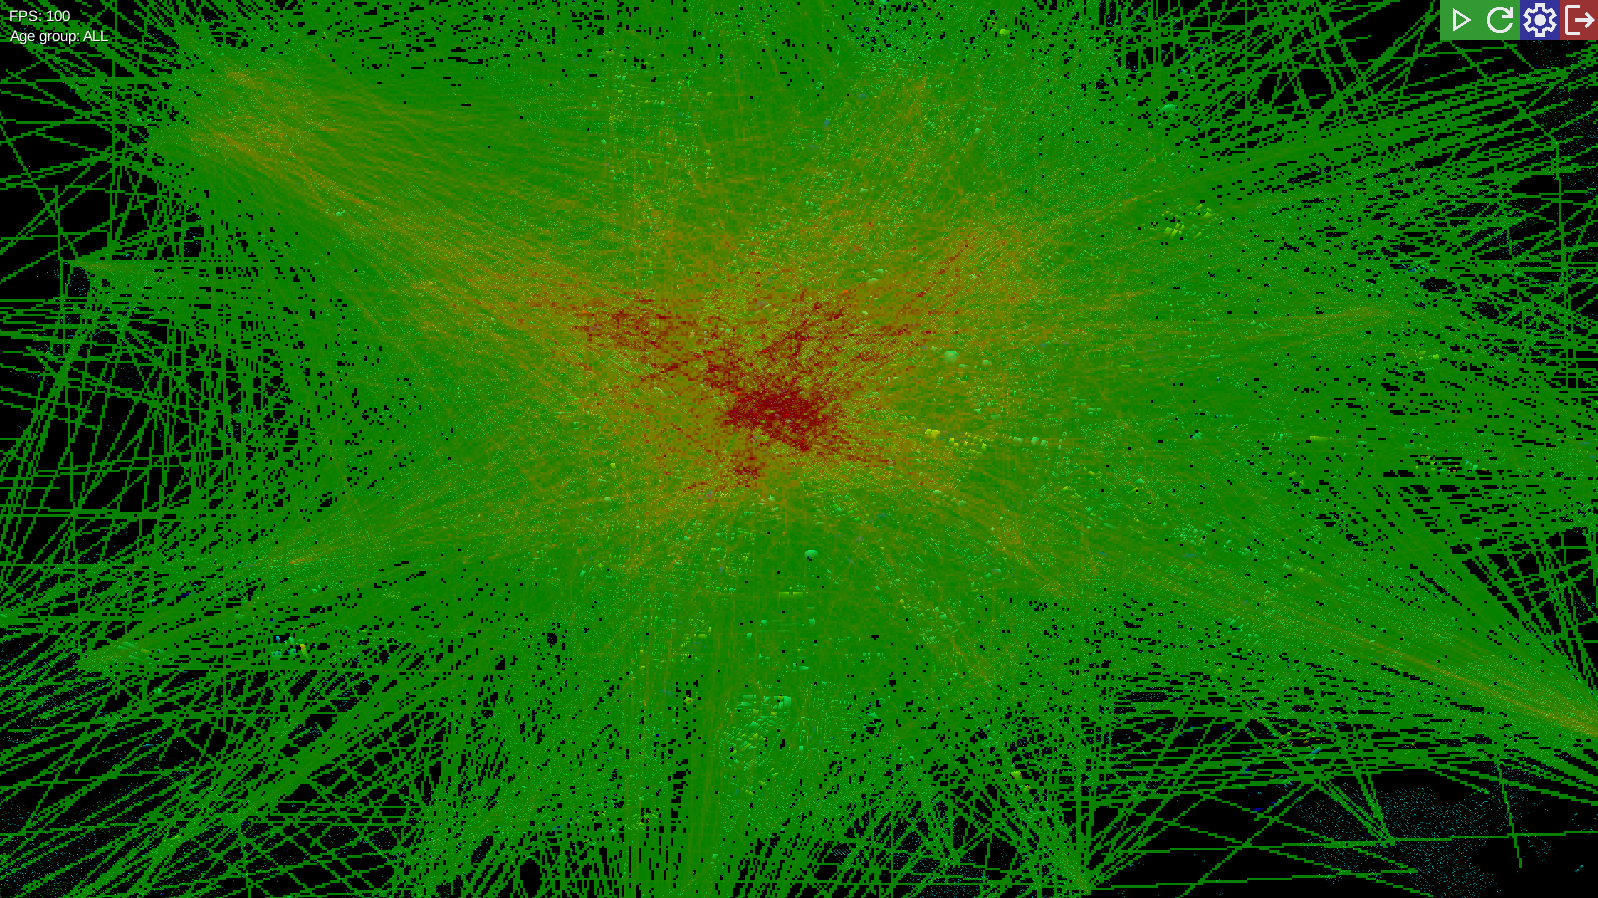
\includegraphics[width=140mm, keepaspectratio]{images/heatmap_5000.png}
    \caption{Heatmap using 5000 agents, see \ref{perftesting-heatmap}}
\end{figure}
\begin{figure}[h]
    \centering
    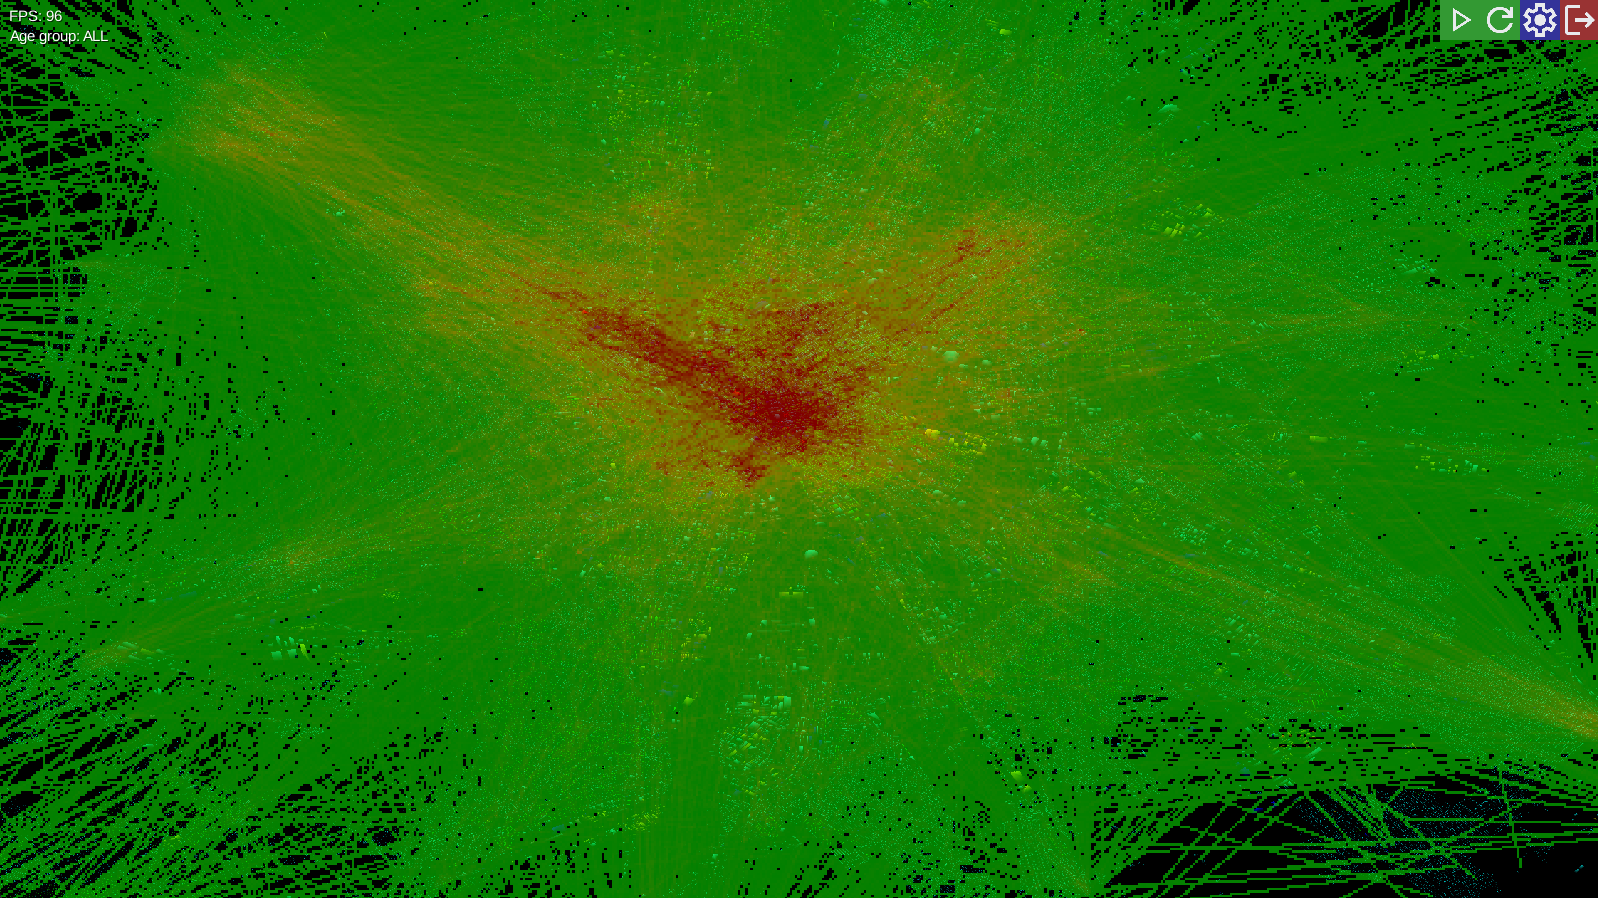
\includegraphics[width=140mm, keepaspectratio]{images/heatmap_10000.png}
    \caption{Heatmap using 10000 agents, see \ref{perftesting-heatmap}}
\end{figure}
\begin{figure}[h]
    \centering
    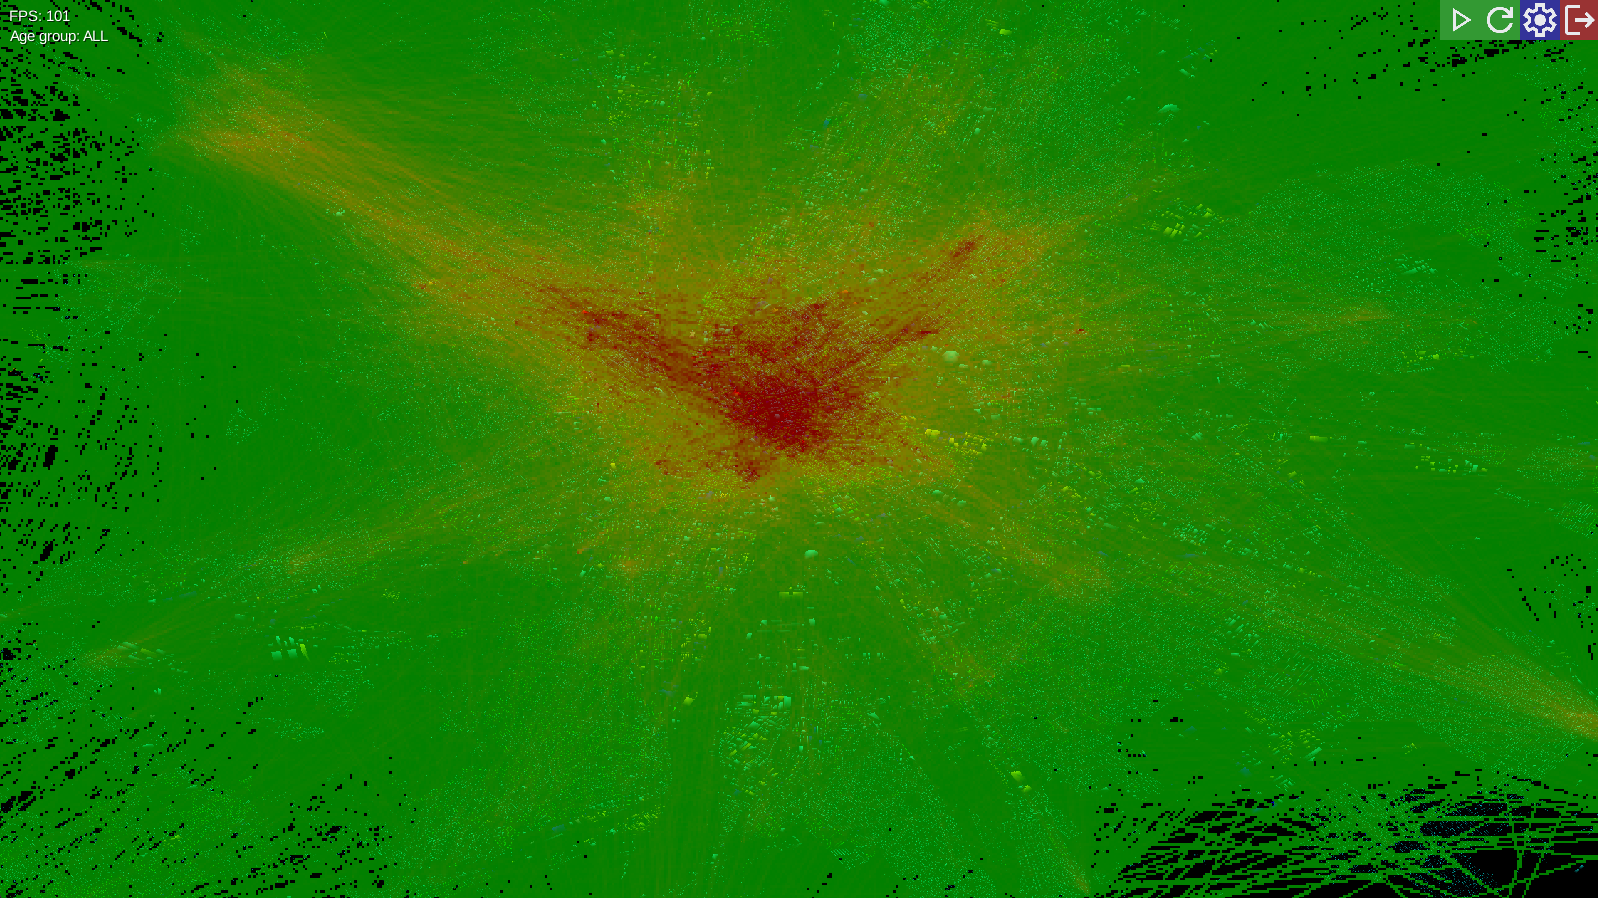
\includegraphics[width=140mm, keepaspectratio]{images/heatmap_20000.png}
    \caption{Heatmap using 20000 agents, see \ref{perftesting-heatmap}}
\end{figure}
\begin{figure}[h]
    \centering
    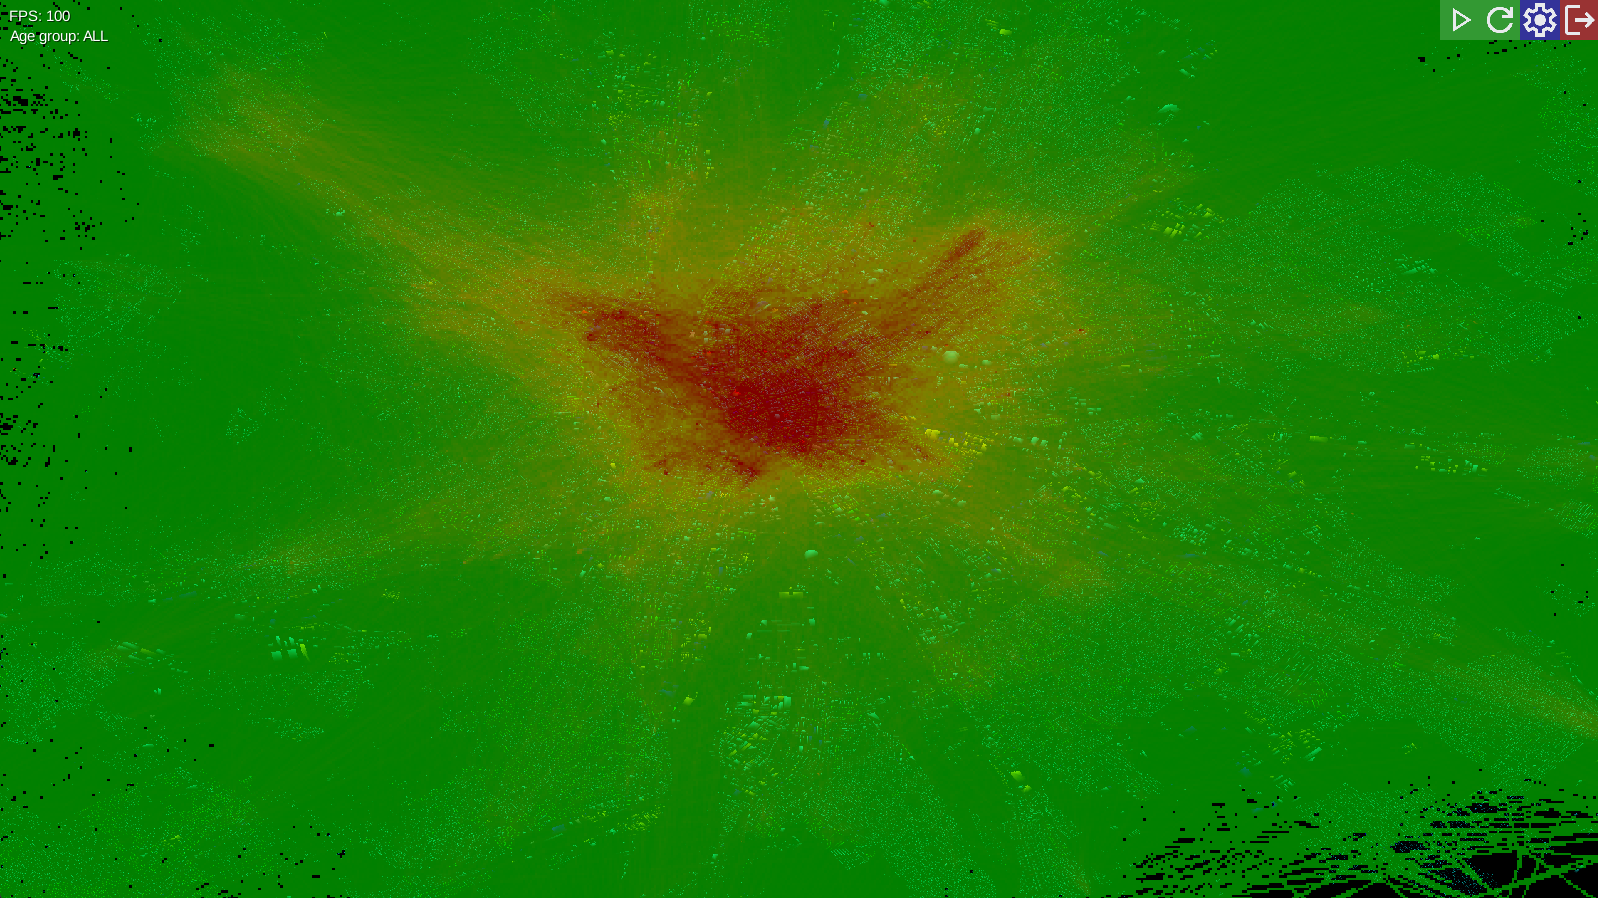
\includegraphics[width=140mm, keepaspectratio]{images/heatmap_50000.png}
    \caption{Heatmap using 50000 agents, see \ref{perftesting-heatmap}}
\end{figure}